\documentclass[12pt,a4paper]{article}

% ── Packages ────────────────────────────────────────────────────────────────
\usepackage[margin=1in]{geometry}
\usepackage{graphicx}
\usepackage{subcaption}
\usepackage{indentfirst}
\usepackage[table,xcdraw]{xcolor}
\usepackage{colortbl}
\usepackage{caption}
\usepackage{fancyhdr}
\usepackage{biblatex}
\usepackage{tikz}
\usepackage{longtable}
\usepackage{array}
\usepackage{booktabs}
\usepackage{multirow}
\usepackage{float}
\usepackage{hyperref}
\usepackage{enumitem}
\usetikzlibrary{arrows.meta,positioning,shapes.geometric,fit,calc,trees}

\addbibresource{sample.bib}

\hypersetup{colorlinks=true,linkcolor=black,citecolor=black,urlcolor=blue}

% ── Page style ───────────────────────────────────────────────────────────────
\pagestyle{fancy}
\fancyhf{}
\fancyhead[R]{\leftmark}
\fancyfoot[C]{\thepage}
\setlength{\headheight}{15pt}

% ── Spacing ──────────────────────────────────────────────────────────────────
\setlength{\parindent}{15pt}
\setlength{\parskip}{0.5em}
\renewcommand{\baselinestretch}{1.15}
\setlist[itemize]{topsep=4pt,itemsep=3pt}

% ── Placeholder box (shows a labeled grey box when the image file is absent) ─
\newcommand{\figplaceholder}[2][6cm]{%
  \noindent\colorbox{gray!12}{\begin{minipage}[c][#1][c]{\dimexpr\linewidth-2\fboxsep}
    \centering\color{gray!60}\small\itshape #2
  \end{minipage}}}

% ── TikZ styles ──────────────────────────────────────────────────────────────
\tikzset{
  block/.style    ={draw,rounded corners,align=center,minimum width=2.7cm,minimum height=1cm,fill=blue!8},
  service/.style  ={draw,rounded corners,align=center,minimum width=3.0cm,minimum height=1cm,fill=green!10},
  data/.style     ={draw,cylinder,shape border rotate=90,aspect=0.25,align=center,
                    minimum height=1cm,minimum width=1.8cm,fill=orange!12},
  actor/.style    ={draw,ellipse,align=center,minimum width=2.2cm,minimum height=0.9cm,fill=purple!10},
  arrow/.style    ={-{Latex[length=2.5mm]},thick},
  entity/.style   ={draw,rounded corners,fill=orange!10,align=left,font=\scriptsize,text width=3.3cm},
  classbox/.style ={draw,rounded corners,fill=cyan!8,align=left,font=\scriptsize,text width=3.5cm}
}

% ════════════════════════════════════════════════════════════════════════════
\begin{document}

% ── Title page ───────────────────────────────────────────────────────────────
\begin{titlepage}
\centering
\IfFileExists{logo.png}{
\includegraphics[width=0.4\textwidth]{logo.png}\par\vspace{0.6cm}}{\vspace*{1cm}}

{\fontsize{18}{22}\selectfont ISS 396 -- Junior Project\par}
{\fontsize{18}{22}\selectfont Final Report\par}

\vspace{1.2cm}\hrule\vspace{1.2cm}

{\fontsize{24}{28}\selectfont \textbf{MyPath}\par}
\vspace{0.3cm}
{\fontsize{15}{19}\selectfont An AI-Powered Career Recommendation and Guidance Platform\par}

\vspace{1.2cm}\hrule\vspace{1cm}

{\fontsize{16}{20}\selectfont Prepared by:\par}\vspace{0.4cm}
{\fontsize{13}{16}\selectfont BENABDA Mohamed Bechir,\quad BENAMMAR Nabila\par}
{\fontsize{13}{16}\selectfont BETTAIEB Mohamed,\quad CHAABEN Baya,\quad SIALA Ghassen\par}

\vspace{1.2cm}
{\fontsize{16}{20}\selectfont Supervised by:\par}\vspace{0.4cm}
{\fontsize{13}{16}\selectfont Mr. BEN MBAREK, Amine -- MedTech\par}

\vfill
{\fontsize{13}{16}\selectfont Tunis, 2025--2026\par}
\end{titlepage}

\tableofcontents\newpage
\listoffigures\newpage
\listoftables\newpage

% ════════════════════════════════════════════════════════════════════════════
\section{Project Overview}

MyPath is an AI-powered career recommendation system that bridges the gap between users' current skills, interests, and aspirations and the rapidly evolving demands of the job market. By combining user input, CV analysis, and intelligent recommendation techniques, the system provides career suggestions, identifies skill gaps, and proposes structured development roadmaps.

\subsection{Introduction}

Choosing an appropriate career path is a critical decision that significantly impacts an individual's future. Many students and young professionals face uncertainty due to a lack of personalized guidance, limited access to professional counseling, and insufficient awareness of available opportunities. Traditional career guidance methods are often generic, time-consuming, and not scalable to meet growing demand.

With the rapid advancement of Artificial Intelligence, new opportunities have emerged to provide intelligent, data-driven, and personalized career guidance. AI systems are capable of analyzing user profiles, extracting meaningful insights from data, and generating tailored recommendations based on individual skills, interests, and goals.

In this context, the \textbf{MyPath} project leverages AI technologies to develop an intelligent career recommendation system that assists users in identifying suitable career paths, analyzing their current competencies, and generating structured roadmaps to achieve their professional objectives. Beyond a simple recommendation interface, MyPath is conceived as a decision-support platform that combines deterministic software engineering mechanisms with AI-assisted reasoning to improve recommendation quality while preserving traceability and user trust.

\subsection{Problem Definition}

Many students and job seekers struggle to identify suitable career paths for several reasons. Most available resources provide generic advice rather than guidance tailored to individual profiles. Users often have difficulty understanding their own skills and how they align with different career opportunities. The rapidly evolving job market makes it difficult to keep track of in-demand skills and emerging professions.

There is therefore a need for an intelligent system capable of: (i)~collecting heterogeneous user data, (ii)~transforming these data into structured profile features, (iii)~comparing the resulting profile with career knowledge, (iv)~explaining the rationale of recommendations, and (v)~translating recommendations into concrete learning actions.

\subsection{Project Objectives}

The principal objective of MyPath is to provide a coherent platform that supports users from initial self-assessment to concrete career planning. This objective is decomposed into the following operational goals:

\begin{itemize}
  \item collect user information through authentication, CV upload, and an adaptive quiz;
  \item extract structured profile data such as skills, education, and interests;
  \item compute ranked career recommendations using a controlled hybrid recommendation pipeline;
  \item identify skill gaps between the current profile and target career requirements;
  \item generate personalized roadmaps that guide users toward realistic next steps; and
  \item facilitate mentor interaction to complement automated guidance with human expertise.
\end{itemize}

\subsection{Project Description}

MyPath is an AI-powered career recommendation platform designed to assist students and job seekers in making informed, personalized career decisions. The system collects and analyzes user data through interactive questionnaires and CV processing, enabling a comprehensive understanding of each user's profile including skills, interests, and academic or professional background.

Using AI techniques such as natural language processing for CV parsing and intelligent recommendation algorithms, the platform extracts relevant information, evaluates user competencies, and matches them with suitable career paths. An adaptive career quiz evolves based on user responses, ensuring more accurate and personalized results.

The system identifies skill gaps by comparing the user's current abilities with the requirements of targeted careers, and provides actionable recommendations. Structured learning and career roadmaps outline the necessary steps, resources, and milestones needed to achieve professional goals. Users can also connect with experienced professionals and schedule mentorship appointments.

The platform is built using modern web and mobile technologies, integrating a responsive React Native frontend, a scalable Python backend, and AI-driven modules to deliver a seamless, interactive, and intelligent user experience.

\subsection{Vulnerabilities and Existing Solutions}

Several career guidance platforms and tools exist today, including online career quizzes, job listing websites, and professional networking platforms. While these solutions provide some level of assistance, they present notable limitations.

Many existing systems rely on static questionnaires that do not adapt to user responses, leading to generic recommendations. Job listing platforms mainly display available opportunities without guiding users on how to acquire required skills. Professional networking platforms allow users to showcase profiles but do not provide in-depth analysis or personalized career planning.

Furthermore, most existing solutions lack advanced analytical capabilities such as automated CV parsing, skill extraction, and gap analysis. Users are rarely informed about which specific skills they are missing for a target career. These limitations highlight the need for a more intelligent, adaptive, and comprehensive solution.

\subsection{Proposed Solution}

To address these challenges, MyPath proposes an AI-powered career recommendation system that delivers personalized and data-driven guidance. The system integrates natural language processing for CV analysis and machine learning techniques for recommendation generation. A key design principle is the use of a \emph{hybrid} architecture: deterministic modules handle state management, scoring, filtering, and persistence, while AI models are used selectively for semantic extraction, profile interpretation, and natural-language explanation.

This separation improves system reliability because essential decisions remain controllable and testable, while AI contributes personalization only where it adds clear value. Additionally, MyPath provides structured roadmaps outlining the steps required to achieve desired career paths, along with identified skill gaps and relevant learning resources.

\subsection{Literature Review}

\subsubsection*{Overview of Career Recommendation Systems}

Career Recommendation Systems (CRSs) have emerged as a growing research area at the intersection of artificial intelligence, information retrieval, and human-computer interaction. Their primary goal is to assist individuals in identifying professional paths that match their skills, interests, experience, and market demand. Unlike general-purpose recommendation systems such as those used in e-commerce or media streaming, CRSs must handle highly heterogeneous data, including textual resumes, free-form interests, structured work histories, and evolving job market signals~\cite{jobrec_arxiv2021}. This complexity has driven the adoption of increasingly sophisticated AI methods to improve both the accuracy and the relevance of career guidance.

\subsubsection*{Core Recommendation Techniques}

Three families of recommendation techniques dominate the literature. \textbf{Content-based filtering} constructs a profile for each user based on explicit attributes such as skills, educational background, and stated preferences, and then matches this profile against item features extracted from job descriptions or career definitions~\cite{ndolo2023job}. This approach is interpretable and performs well when rich user data is available, but it tends to over-specialize recommendations because it relies entirely on the user's own history and may fail to suggest unexpected but suitable alternatives.

\textbf{Collaborative filtering} addresses this limitation by identifying users with similar behavior patterns and recommending items that analogous users found relevant~\cite{maan2018hybrid}. Memory-based variants compute user-to-user or item-to-item similarities directly, while model-based variants apply matrix factorization, neural embeddings, or probabilistic models to capture latent preference structures. The main drawback of collaborative filtering in career systems is the cold-start problem: newly registered users or recently created job profiles have insufficient interaction data to yield reliable similarity scores~\cite{springer2022job}.

\textbf{Knowledge-based approaches} use a formal representation of career domain knowledge, for example a taxonomy of skills or an ontology of professional roles, to reason about the suitability of a career for a given user without relying on historical interaction data~\cite{ndolo2023job}. These systems are particularly valuable in low-data situations and offer strong explainability because each recommendation can be traced to specific rules or domain facts. However, maintaining a comprehensive and current knowledge base requires significant ongoing effort.

Given the limitations of each individual approach, the majority of recent CRSs adopt \textbf{hybrid architectures} that combine two or more techniques~\cite{ndolo2023job, jobrec_arxiv2021}. A common pattern is to use content-based filtering to compute an initial candidate set and then apply collaborative signals or knowledge-based re-ranking to refine the results. Hybrid systems consistently outperform single-method approaches in benchmark evaluations, particularly on diversity and coverage metrics.

\subsubsection*{Natural Language Processing and Resume Analysis}

Text mining and natural language processing have become central components in modern career recommendation pipelines~\cite{jobrec_arxiv2021}. The ability to extract structured information from unstructured documents such as resumes and job postings is a prerequisite for accurate profile-to-career matching. Classical approaches relied on rule-based parsers and keyword extraction with predefined ontologies. More recent work has shifted toward transformer-based language models such as BERT and its domain-specific variants, which can perform named entity recognition, skill classification, and semantic similarity comparison in an end-to-end trainable manner.

Skill extraction is one of the most studied tasks in this context. Research has shown that a significant proportion of skills mentioned in resumes and job descriptions do not appear in standard skill taxonomies such as O*NET or ESCO, making exact-match approaches insufficient~\cite{jobrec_arxiv2021}. Semantic embedding methods, which represent skills as dense vectors in a shared latent space, allow the system to identify near-equivalent skills and capture hierarchical relationships between competencies. These representations also support skill gap analysis, in which the distance between a user's current skill vector and a target career's required skill vector is computed to identify which competencies need to be developed.

\subsubsection*{Deep Learning and Generative AI in Career Guidance}

Recent years have seen a rapid transition toward deep learning architectures in recommender systems more broadly, with a growing number of applications in career guidance~\cite{jobrec_arxiv2021}. Graph neural networks have been applied to model the complex relationships between users, skills, jobs, and industries, capturing structural dependencies that are invisible to flat feature-based methods. Recurrent and attention-based models have been used to model career trajectories as temporal sequences, enabling systems to recommend not just a single career but an ordered progression of roles.

The emergence of large language models (LLMs) has introduced a new paradigm for career guidance. LLMs can generate natural-language explanations for recommendations, engage users in conversational career exploration, and produce structured learning roadmaps in response to free-form prompts. However, deploying LLMs in production career systems raises important concerns around hallucination, bias amplification, and lack of controllability~\cite{springer2022job}. Retrieval-Augmented Generation (RAG) has been proposed as a mitigation strategy: instead of relying on the model's parametric knowledge alone, the system retrieves relevant facts from a controlled knowledge base and conditions the generation on that retrieved context, thereby grounding the output in verifiable information.

\subsubsection*{Open Challenges}

Despite substantial progress, several challenges remain unresolved in the literature. \textbf{Fairness and bias} are major concerns because recommendation systems trained on historical labor market data may reinforce existing inequalities, for example by under-recommending high-paying technical roles to users from underrepresented groups~\cite{springer2022job}. \textbf{Context awareness} is another limitation: most systems treat user profiles as static snapshots and do not account for dynamic factors such as geographic location, economic conditions, or short-term skill trends that strongly influence career outcomes. The \textbf{cold-start problem} remains difficult to fully resolve, particularly for new users who have not yet uploaded a CV or completed any quiz, and for newly created career profiles that have no historical interaction data~\cite{springer2022job}. Finally, most existing systems focus on recommendation accuracy at the expense of \textbf{explainability}: they generate a list of suggested careers without providing the user with a clear rationale or an actionable path forward.

\subsubsection*{Positioning of MyPath}

MyPath builds upon the insights from this body of research while addressing its key limitations. The platform adopts a hybrid recommendation architecture that combines deterministic profile-to-career scoring with AI-generated explanations, thereby achieving both reliability and personalization. CV analysis is performed using NLP-based skill extraction, and the resulting structured profile is used jointly with adaptive quiz responses to compute a comprehensive user feature vector. A Hybrid Modular RAG pipeline is used for roadmap generation, grounding personalized learning plans in a curated internal knowledge base rather than relying on unconstrained generative output. These design choices are directly motivated by the open challenges identified in the literature: the hybrid architecture improves on single-method baselines, the RAG design reduces hallucination risk, and the deterministic scoring layer preserves explainability and auditability throughout the recommendation process.

\subsection{Conclusion}

This chapter provided a comprehensive overview of the MyPath project. The introduction established the context by highlighting the growing demand for intelligent and personalized career guidance, and the inadequacy of traditional counseling methods to meet that demand at scale. The problem definition identified the five core requirements that a useful career guidance platform must fulfill: heterogeneous data collection, structured profile extraction, profile-to-career comparison, recommendation explainability, and translation of results into actionable learning steps.

The project objectives were formulated as a coherent set of operational goals spanning the full user journey, from initial authentication and CV upload to mentor interaction and progress tracking. The project description presented the overall structure of the platform and the key technologies involved. The analysis of existing solutions revealed recurring weaknesses — static questionnaires, absence of skill gap analysis, and lack of explainability — that justify the development of a more intelligent and adaptive system.

The proposed solution introduced the hybrid design principle that underpins MyPath: deterministic modules ensure that core decisions are controllable, testable, and explainable, while AI-assisted components contribute personalization and natural-language generation selectively. The literature review contextualized this approach within the broader research landscape, surveying content-based, collaborative, knowledge-based, and hybrid recommendation techniques, NLP-driven resume analysis, the emergence of LLMs and RAG in career guidance, and the open challenges around fairness, cold-start, context-awareness, and explainability.

Taken together, the elements presented in this chapter establish both the need for MyPath and the scientific justification for its design choices. The following chapters translate these insights into concrete system specifications, a detailed technical design, and a functional implementation, providing a complete engineering account of the proposed solution.

\clearpage

% ════════════════════════════════════════════════════════════════════════════
\section{Product Specifications}

This chapter translates user needs into technical requirements that are measurable, testable, and aligned with the problem domain. It outlines the project plan, features, requirements, standards, and constraints that shape the final product.

\subsection{Introduction}

The specification of the MyPath system is based on a thorough analysis of user needs and system objectives. It defines clear functional and non-functional requirements that guide the design and development of the platform. A structured project management approach based on the Scrum methodology is adopted to organize and manage these requirements throughout the development lifecycle.

\subsection{Project Management}

\subsubsection{Methodology}

The MyPath project adopts the Scrum methodology, an agile framework that manages complex projects in a flexible and iterative manner through short development cycles called sprints. The product backlog contains all identified user stories and requirements, prioritized by impact. For each sprint, a subset forms the sprint backlog defining the tasks to be completed within that iteration.

Jira is used as a project management tool to organize and track tasks, monitor sprint progress, and visualize workflows. Regular Scrum ceremonies, including sprint planning, reviews, and retrospectives, are conducted every one to two weeks to ensure effective collaboration and continuous progress.

\subsubsection{Timeline}

The development of MyPath is organized into six iterative sprints, each lasting one to two weeks and focusing on a specific set of functionalities.

\begin{table}[H]
\centering
\begin{tabular}{|c|c|c|}
\hline
\textbf{Sprint} & \textbf{From} & \textbf{To} \\
\hline
Sprint 1 & Week 1  & Week 2  \\
Sprint 2 & Week 3  & Week 4  \\
Sprint 3 & Week 5  & Week 6  \\
Sprint 4 & Week 7  & Week 8  \\
Sprint 5 & Week 9  & Week 10 \\
Sprint 6 & Week 11 & Week 12 \\
\hline
\end{tabular}
\caption{Sprints Planning}
\end{table}

\subsection{Product Backlog}

\begin{table}[H]
\centering
\begin{tabular}{|p{9.5cm}|c|}
\hline
\textbf{User Story} & \textbf{Priority} \\
\hline
\textbf{Sprint 1:} User registration, account creation, login and authentication & High \\
\hline
\textbf{Sprint 2:} CV upload, PDF parsing, skill and experience extraction & High \\
\hline
\textbf{Sprint 3:} Adaptive quiz engine, session management, user profiling & High \\
\hline
\textbf{Sprint 4:} Career recommendation pipeline, hybrid scoring, result persistence & High \\
\hline
\textbf{Sprint 5:} Skill gap analysis, learning roadmap generation via RAG pipeline & Medium \\
\hline
\textbf{Sprint 6:} Mentor browsing, appointment scheduling, job board integration & Medium \\
\hline
\end{tabular}
\caption{Product Backlog}
\end{table}

\subsection{Sprint Backlog}

The sprint backlog specifies the user stories and tasks selected for each iteration. Each sprint is tracked in Jira, where tasks are organized, assigned, and monitored throughout the sprint lifecycle.

\subsubsection{Sprint 1}

\begin{figure}[H]
  \centering
  \IfFileExists{figures/sprint1.png}{
    \includegraphics[width=\linewidth]{figures/sprint1.png}
  }{\figplaceholder[5cm]{Insert Sprint 1 Jira backlog screenshot\\(authentication and account creation tasks)}}
  \caption{Sprint 1 Backlog}
\end{figure}

\subsubsection{Sprint 2}

\begin{figure}[H]
  \centering
  \IfFileExists{figures/sprint2.png}{
    \includegraphics[width=\linewidth]{figures/sprint2.png}
  }{\figplaceholder[5cm]{Insert Sprint 2 Jira backlog screenshot\\(CV upload and parsing tasks)}}
  \caption{Sprint 2 Backlog}
\end{figure}

\subsubsection{Sprint 3}

\begin{figure}[H]
  \centering
  \IfFileExists{figures/sprint3.png}{
    \includegraphics[width=\linewidth]{figures/sprint3.png}
  }{\figplaceholder[5cm]{Insert Sprint 3 Jira backlog screenshot\\(adaptive quiz engine tasks)}}
  \caption{Sprint 3 Backlog}
\end{figure}

\subsubsection{Sprint 4}

\begin{figure}[H]
  \centering
  \IfFileExists{figures/sprint4.png}{
    \includegraphics[width=\linewidth]{figures/sprint4.png}
  }{\figplaceholder[5cm]{Insert Sprint 4 Jira backlog screenshot\\(recommendation pipeline tasks)}}
  \caption{Sprint 4 Backlog}
\end{figure}

\subsubsection{Sprint 5}

\begin{figure}[H]
  \centering
  \IfFileExists{figures/sprint5.png}{
    \includegraphics[width=\linewidth]{figures/sprint5.png}
  }{\figplaceholder[5cm]{Insert Sprint 5 Jira backlog screenshot\\(roadmap and skill gap tasks)}}
  \caption{Sprint 5 Backlog}
\end{figure}

\subsubsection{Sprint 6}

\begin{figure}[H]
  \centering
  \IfFileExists{figures/sprint6.png}{
    \includegraphics[width=\linewidth]{figures/sprint6.png}
  }{\figplaceholder[5cm]{Insert Sprint 6 Jira backlog screenshot\\(mentor and job board tasks)}}
  \caption{Sprint 6 Backlog}
\end{figure}

\subsection{Requirements Specification}

\subsubsection{Functional Requirements}

The functional requirements describe the core features and operations the system must provide to its users.

\subsubsection*{Use Case Scenarios}

\begin{itemize}
  \item \textbf{Account Creation:} A user registers on the platform to access personalized features.
  \item \textbf{User Authentication:} A user logs into the system securely using their credentials.
  \item \textbf{CV Upload and Analysis:} A user uploads their CV; the system extracts relevant skills and information.
  \item \textbf{Dynamic Quiz Completion:} A user completes an adaptive quiz that progressively refines their profile.
  \item \textbf{Career Recommendation:} The system provides personalized career suggestions based on user data.
  \item \textbf{Skill Gap Identification:} The system identifies missing skills required for selected career paths.
  \item \textbf{Roadmap Generation:} The system generates a structured learning roadmap to guide the user.
  \item \textbf{Mentor Interaction:} A user connects with a mentor and schedules an appointment for personalized guidance.
\end{itemize}

\subsubsection*{Use Case Diagram}

\begin{figure}[H]
  \centering
  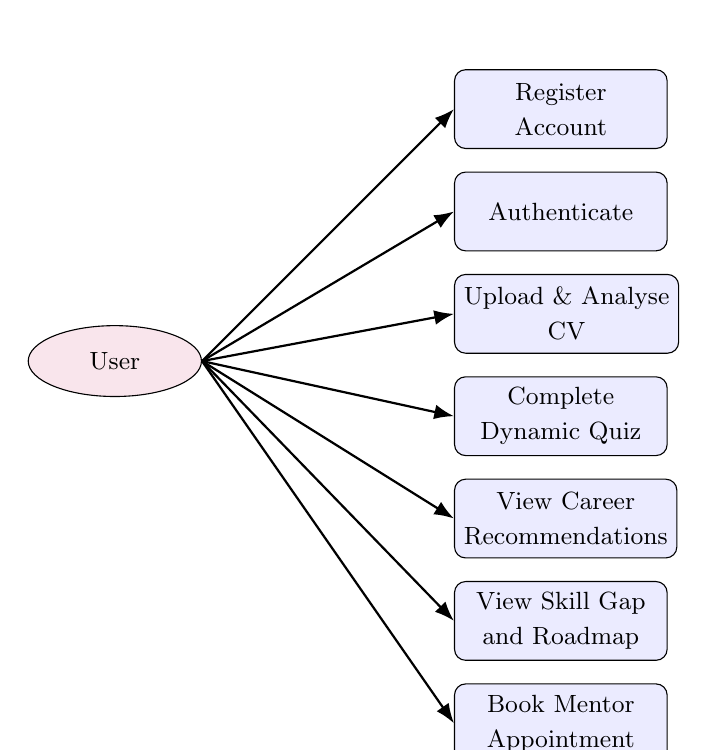
\begin{tikzpicture}[node distance=0.9cm and 1.6cm, every node/.style={font=\small}]
    \node[actor] (user) {User};
    \node[block, right=3.2cm of user, yshift= 3.2cm] (register)  {Register\\Account};
    \node[block, right=3.2cm of user, yshift= 1.9cm] (login)     {Authenticate};
    \node[block, right=3.2cm of user, yshift= 0.6cm] (cv)        {Upload \& Analyse\\CV};
    \node[block, right=3.2cm of user, yshift=-0.7cm] (quiz)      {Complete\\Dynamic Quiz};
    \node[block, right=3.2cm of user, yshift=-2.0cm] (recommend) {View Career\\Recommendations};
    \node[block, right=3.2cm of user, yshift=-3.3cm] (roadmap)   {View Skill Gap\\and Roadmap};
    \node[block, right=3.2cm of user, yshift=-4.6cm] (mentor)    {Book Mentor\\Appointment};
    \foreach \x in {register,login,cv,quiz,recommend,roadmap,mentor}
      \draw[arrow] (user.east) -- (\x.west);
  \end{tikzpicture}
  \caption{Use Case Diagram of MyPath}
\end{figure}

\subsubsection{Non-functional Requirements}

\begin{itemize}
  \item \textbf{Performance:} The system should respond within two seconds for standard user interactions; recommendation generation may take up to five seconds.
  \item \textbf{Scalability:} The platform should handle a growing number of users without performance degradation.
  \item \textbf{Usability:} The system should offer an intuitive, accessible interface suitable for a wide range of users.
  \item \textbf{Security:} User data must be securely stored and protected, ensuring confidentiality and integrity.
  \item \textbf{Reliability:} The system should operate consistently with minimal downtime.
  \item \textbf{Maintainability:} The system should follow a modular design to facilitate updates and extensions.
\end{itemize}

\subsection{Project Considerations}

\subsubsection{Project Constraints}

The development of MyPath is subject to time constraints imposed by the academic schedule, technical constraints related to computing resources and external API access, and team-size constraints that affect task distribution and development speed. These constraints require careful prioritization to ensure essential features are delivered on time.

\subsubsection{Project Limitations}

The accuracy of career recommendations depends on the quality and completeness of user-provided data. In cases where input is limited or inaccurate, recommendation quality may decrease. The system may also not fully capture all aspects of the dynamic job market, and some advanced features may be constrained by available resources.

\subsubsection{Project Delimitations}

MyPath primarily targets students and early-career job seekers. The project does not include direct integration with recruitment platforms or real-time job application systems. It focuses on recommendation, analysis, and guidance features to deliver a well-defined solution within its scope.

\subsubsection{Project Assumptions}

It is assumed that users provide accurate and relevant information when interacting with the system, that users are interested in receiving personalized career guidance, and that mentors participating in the platform are qualified and available to provide meaningful guidance.

\subsubsection{Project Standards}

MyPath follows Agile principles for project management and adheres to standard coding conventions to ensure maintainability. Security standards including proper authentication, encrypted storage, and secure data transmission are applied throughout the system.

\subsubsection{Business, Social and Ethical Considerations}

From a business perspective, the platform supports users in making better career decisions, improving employability. Socially, it promotes equal access to career guidance by providing an accessible and scalable solution to those without professional counseling resources. Ethically, the system must ensure fairness and avoid bias in recommendations. User data must be handled responsibly and with transparency about how recommendations are generated, in order to build trust and ensure responsible use.

\subsection{Conclusion}

This chapter presented the specifications of MyPath, including functional and non-functional requirements, the project management approach, and key project considerations. These specifications provide a structured foundation for the design and development of the system presented in the following chapter.

\clearpage

% ════════════════════════════════════════════════════════════════════════════
\section{Product Design}

This chapter presents the technical design of the MyPath system, covering the global architecture, database structure, API contract, behavioral models, wireframe interface layout, and security considerations that form the engineering foundation of the platform.

\subsection{Introduction}

The MyPath architecture is designed to support personalized career guidance while ensuring clear separation of concerns between deterministic business logic, persistent data management, and AI-assisted services. Rather than relying entirely on large language models, the system adopts a hybrid design: core decisions are performed through controlled deterministic processes, while AI is used selectively for explanation, personalization, and text generation. This improves robustness and makes system behavior easier to validate, maintain, and extend.

\subsection{High-Level Design}

\subsubsection{Architecture Overview}

The MyPath system follows a layered architecture composed of four principal layers:

\begin{itemize}
  \item The \textbf{Mobile Frontend} (React Native) handles all user interaction including authentication, quiz participation, CV upload, recommendation visualization, roadmap consultation, and mentor scheduling. It communicates exclusively with the backend through secured API endpoints.
  \item The \textbf{Python Backend} acts as the central coordination layer. It implements application logic following the Model--View--Controller pattern, validates requests, manages session state, and invokes AI capabilities only through a controlled orchestration module.
  \item \textbf{Supabase} provides the Backend-as-a-Service infrastructure, offering PostgreSQL-based persistence, JWT authentication, and file storage for CV documents.
  \item The \textbf{AI Orchestration Layer} centralizes prompt handling, reasoning workflows, and output schema validation to prevent uncontrolled AI usage and guarantee that AI outputs remain bounded by application rules.
\end{itemize}

\begin{figure}[H]
  \centering
  \resizebox{\textwidth}{!}{%
  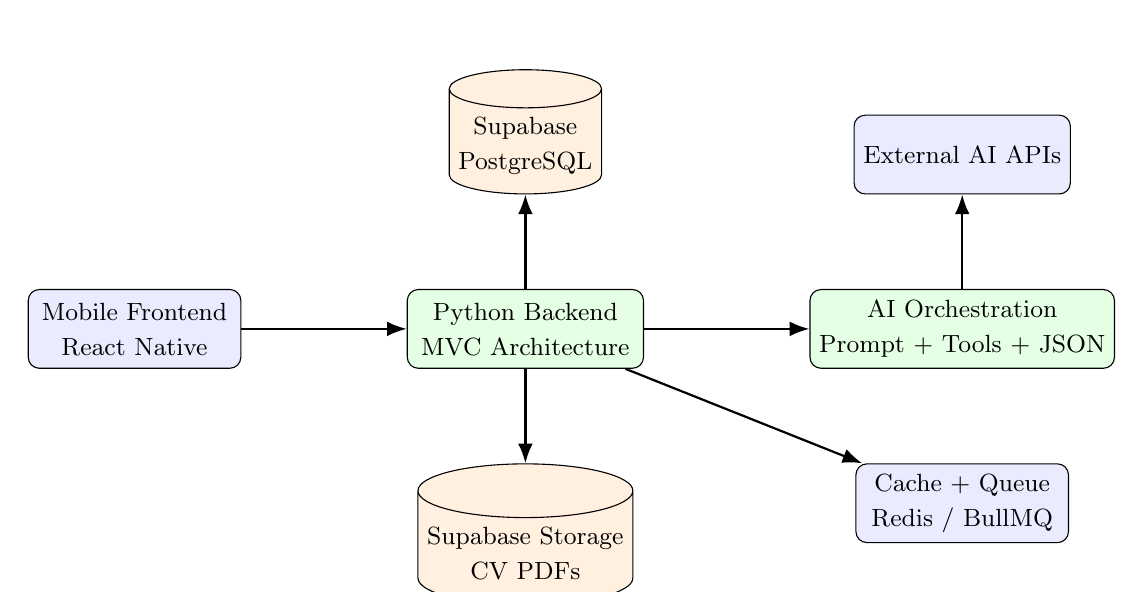
\begin{tikzpicture}[node distance=1.2cm and 1.5cm, every node/.style={font=\small}]
    \node[block]  (frontend) {Mobile Frontend\\React Native};
    \node[service,right=2.1cm of frontend] (backend)  {Python Backend\\MVC Architecture};
    \node[service,right=2.1cm of backend]  (ai)       {AI Orchestration\\Prompt + Tools + JSON};
    \node[data,   above=1.2cm of backend]  (db)       {Supabase\\PostgreSQL};
    \node[data,   below=1.2cm of backend]  (storage)  {Supabase Storage\\CV PDFs};
    \node[block,  above=1.2cm of ai]       (llm)      {External AI APIs};
    \node[block,  below=1.2cm of ai]       (cache)    {Cache + Queue\\Redis / BullMQ};
    \draw[arrow] (frontend) -- (backend);
    \draw[arrow] (backend)  -- (db);
    \draw[arrow] (backend)  -- (storage);
    \draw[arrow] (backend)  -- (ai);
    \draw[arrow] (ai)       -- (llm);
    \draw[arrow] (backend)  -- (cache);
  \end{tikzpicture}}
  \caption{Global architecture of the MyPath system}
\end{figure}

The backend follows the MVC pattern. The \textbf{Model} layer contains data entities and business logic stored in the database. The \textbf{Controller} layer manages incoming requests, validates payloads, coordinates processing pipelines, and invokes AI when required. The \textbf{View} layer corresponds to the structured JSON responses returned to the mobile client.

\subsubsection{AI Orchestration Design}

The AI orchestration layer supervises all interactions with external AI models. AI is not responsible for core decision-making: career ranking, scoring, and persistence are handled by deterministic modules. AI is used only after these modules have produced reliable intermediate results, for example to generate user-facing explanations after the recommendation engine has computed career rankings.

The AI layer combines three model families:
\begin{itemize}
  \item \textbf{Large language models} for explanation generation, roadmap personalization, and text reformulation;
  \item \textbf{Embedding models} for semantic similarity between skills, course descriptions, and career profiles; and
  \item \textbf{Rule-based scoring modules} for deterministic matching, filtering, and confidence control.
\end{itemize}

This hybrid organization improves explainability, control, reliability, and testability compared to a purely generative approach.

\subsubsection{Component Diagram}

\begin{figure}[H]
  \centering
  \resizebox{\textwidth}{!}{%
  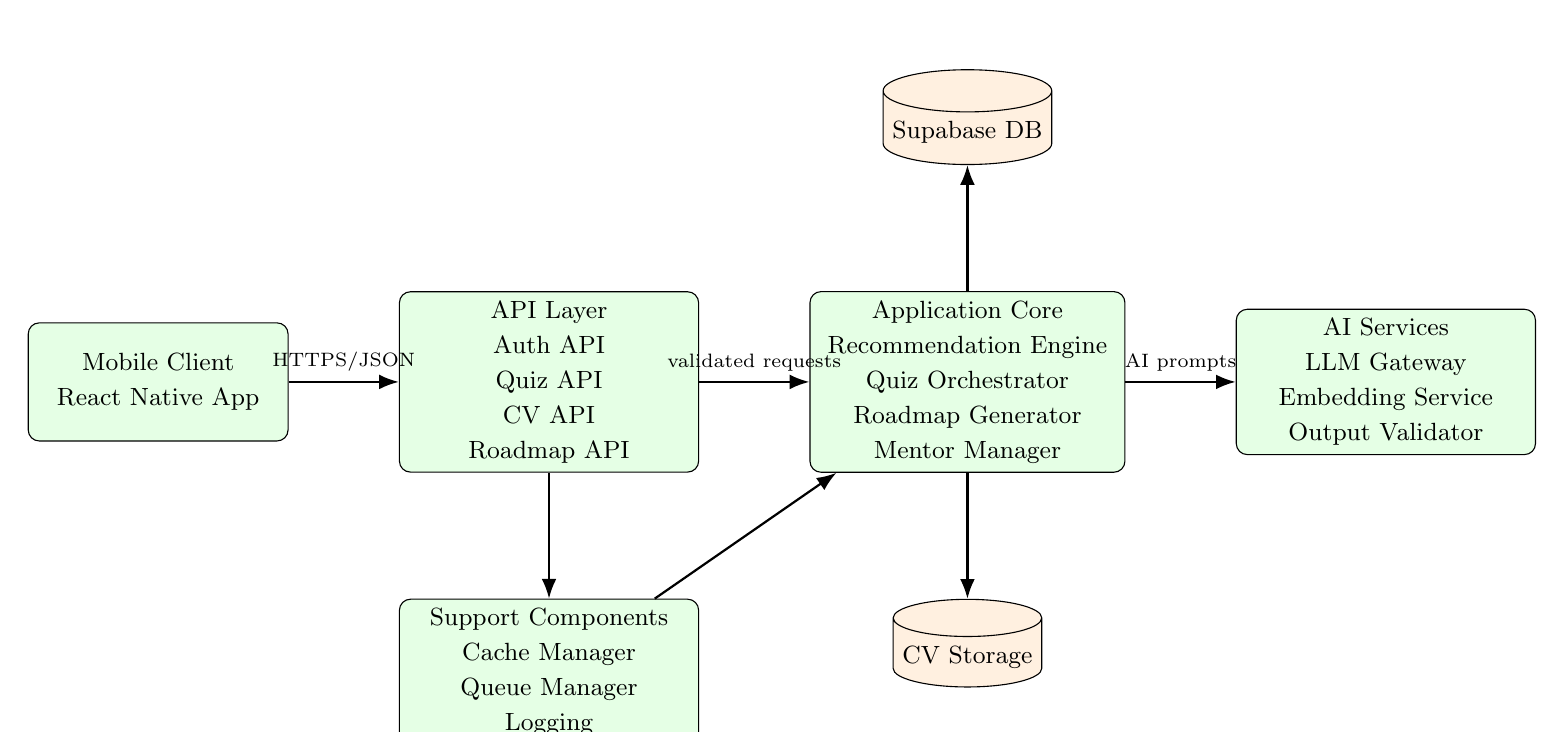
\begin{tikzpicture}[node distance=1.0cm and 1.2cm, every node/.style={font=\small}]
    \node[service,minimum width=3.3cm,minimum height=1.5cm] (frontend) {Mobile Client\\React Native App};
    \node[service,right=1.4cm of frontend,minimum width=3.8cm,minimum height=2.0cm] (api)
      {API Layer\\Auth API\\Quiz API\\CV API\\Roadmap API};
    \node[service,right=1.4cm of api,minimum width=4.0cm,minimum height=2.2cm] (core)
      {Application Core\\Recommendation Engine\\Quiz Orchestrator\\Roadmap Generator\\Mentor Manager};
    \node[data,   above=1.6cm of core]  (db)      {Supabase DB};
    \node[data,   below=1.6cm of core]  (storage) {CV Storage};
    \node[service,right=1.4cm of core,minimum width=3.8cm,minimum height=1.8cm] (ai)
      {AI Services\\LLM Gateway\\Embedding Service\\Output Validator};
    \node[service,below=1.6cm of api,minimum width=3.8cm,minimum height=1.6cm] (support)
      {Support Components\\Cache Manager\\Queue Manager\\Logging};
    \draw[arrow] (frontend) -- node[above,font=\scriptsize]{HTTPS/JSON} (api);
    \draw[arrow] (api)      -- node[above,font=\scriptsize]{validated requests} (core);
    \draw[arrow] (core)     -- node[above,font=\scriptsize]{AI prompts} (ai);
    \draw[arrow] (core)     -- (db);
    \draw[arrow] (core)     -- (storage);
    \draw[arrow] (api)      -- (support);
    \draw[arrow] (support)  -- (core);
  \end{tikzpicture}}
  \caption{Component diagram of the MyPath backend architecture}
\end{figure}

\subsection{Database Design}

The database design of MyPath uses a relational model to preserve referential integrity, session traceability, and structured persistence of recommendation outputs.

\subsubsection{Entity--Relationship Diagram}

\begin{figure}[H]
  \centering
  \resizebox{\textwidth}{!}{%
  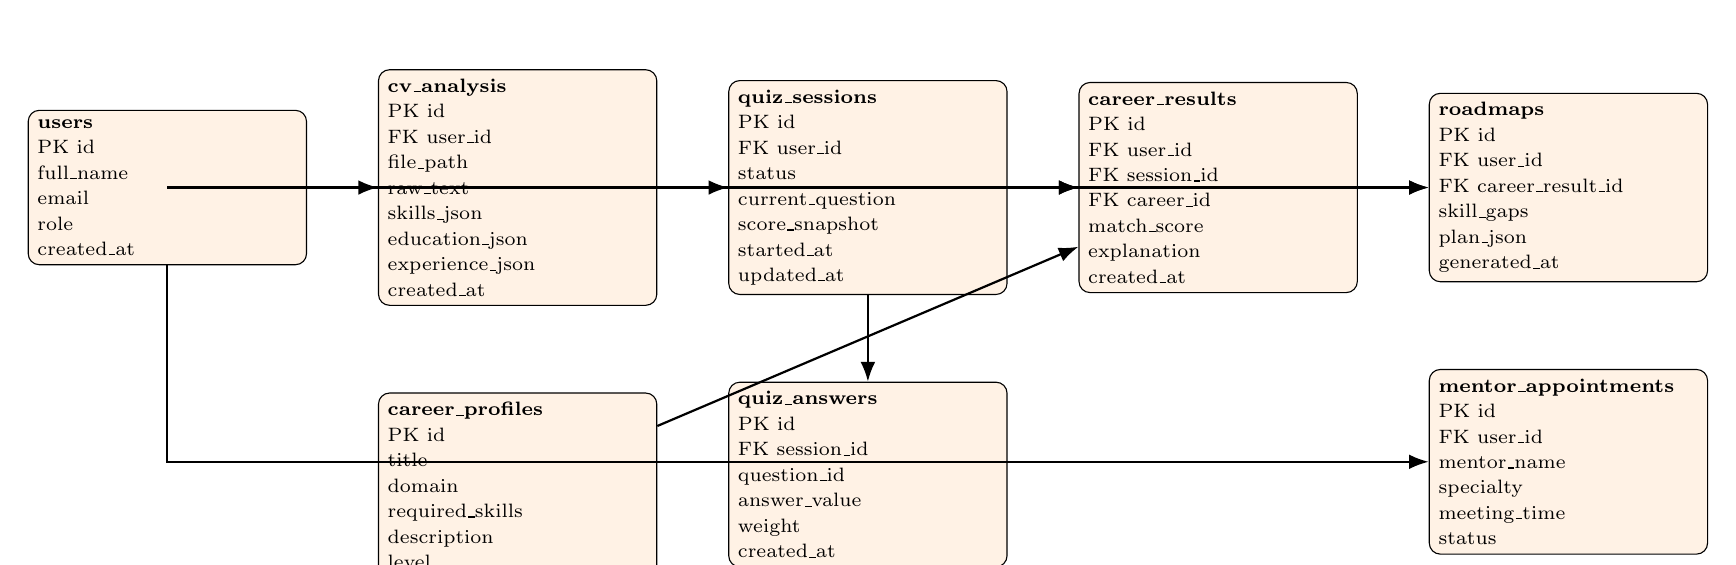
\begin{tikzpicture}[node distance=1.0cm and 0.9cm]
    \node[entity] (users)   {\textbf{users}\\PK id\\full\_name\\email\\role\\created\_at};
    \node[entity,right=0.9cm of users]   (cv)      {\textbf{cv\_analysis}\\PK id\\FK user\_id\\file\_path\\raw\_text\\skills\_json\\education\_json\\experience\_json\\created\_at};
    \node[entity,right=0.9cm of cv]      (quizs)   {\textbf{quiz\_sessions}\\PK id\\FK user\_id\\status\\current\_question\\score\_snapshot\\started\_at\\updated\_at};
    \node[entity,below=1.1cm of quizs]   (answers) {\textbf{quiz\_answers}\\PK id\\FK session\_id\\question\_id\\answer\_value\\weight\\created\_at};
    \node[entity,below=1.1cm of cv]      (careers) {\textbf{career\_profiles}\\PK id\\title\\domain\\required\_skills\\description\\level};
    \node[entity,right=0.9cm of quizs]   (results) {\textbf{career\_results}\\PK id\\FK user\_id\\FK session\_id\\FK career\_id\\match\_score\\explanation\\created\_at};
    \node[entity,right=0.9cm of results] (roadmaps){\textbf{roadmaps}\\PK id\\FK user\_id\\FK career\_result\_id\\skill\_gaps\\plan\_json\\generated\_at};
    \node[entity,below=1.1cm of roadmaps](mentors)  {\textbf{mentor\_appointments}\\PK id\\FK user\_id\\mentor\_name\\specialty\\meeting\_time\\status};
    \draw[arrow] (users)   -- (cv);
    \draw[arrow] (users)   -- (quizs);
    \draw[arrow] (quizs)   -- (answers);
    \draw[arrow] (careers) -- (results);
    \draw[arrow] (users)   |- (results);
    \draw[arrow] (quizs)   -- (results);
    \draw[arrow] (results) -- (roadmaps);
    \draw[arrow] (users)   |- (roadmaps);
    \draw[arrow] (users)   |- (mentors);
  \end{tikzpicture}}
  \caption{Entity--relationship diagram of the MyPath database}
\end{figure}

\subsubsection{Table Descriptions}

\begin{longtable}{|p{3cm}|p{4.2cm}|p{6.8cm}|}
\hline
\textbf{Table} & \textbf{Purpose} & \textbf{Main Attributes} \\
\hline
\texttt{users}               & Stores authenticated user identities and roles.
                             & \texttt{id}, \texttt{full\_name}, \texttt{email}, \texttt{role}, \texttt{created\_at} \\
\hline
\texttt{cv\_analysis}        & Persists uploaded CV metadata and extracted structured content.
                             & \texttt{user\_id}, \texttt{file\_path}, \texttt{skills\_json}, \texttt{education\_json}, \texttt{experience\_json} \\
\hline
\texttt{quiz\_sessions}      & Tracks the progression and state of each quiz attempt.
                             & \texttt{user\_id}, \texttt{status}, \texttt{current\_question}, \texttt{score\_snapshot} \\
\hline
\texttt{quiz\_answers}       & Stores each answer submitted within a quiz session.
                             & \texttt{session\_id}, \texttt{question\_id}, \texttt{answer\_value}, \texttt{weight} \\
\hline
\texttt{career\_profiles}    & Contains normalized career definitions used by the matching engine.
                             & \texttt{title}, \texttt{domain}, \texttt{required\_skills}, \texttt{description}, \texttt{level} \\
\hline
\texttt{career\_results}     & Stores ranked recommendation outputs generated for a user.
                             & \texttt{user\_id}, \texttt{session\_id}, \texttt{career\_id}, \texttt{match\_score}, \texttt{explanation} \\
\hline
\texttt{roadmaps}            & Stores generated learning plans and identified skill gaps.
                             & \texttt{user\_id}, \texttt{career\_result\_id}, \texttt{skill\_gaps}, \texttt{plan\_json} \\
\hline
\texttt{mentor\_appointments}& Manages mentor booking information.
                             & \texttt{user\_id}, \texttt{mentor\_name}, \texttt{specialty}, \texttt{meeting\_time}, \texttt{status} \\
\hline
\caption{Database table descriptions}
\end{longtable}

A single user can upload multiple CVs, start multiple quiz sessions, receive multiple recommendation results, and maintain more than one roadmap over time. This relational structure supports auditability, reproducibility, and future analytics.

\subsection{API Design}

The API layer exposes application capabilities as authenticated REST endpoints, acting as the contract between the mobile frontend and the backend services.

\subsubsection{Main Endpoints}

\begin{table}[H]
\centering\small
\begin{tabular}{|p{4cm}|p{1.8cm}|p{8cm}|}
\hline
\textbf{Endpoint} & \textbf{Method} & \textbf{Purpose} \\
\hline
\texttt{/auth/register}            & POST & Create a new user account. \\
\texttt{/auth/login}               & POST & Authenticate a user and issue an access token. \\
\texttt{/quiz/start}               & POST & Create a new quiz session and return the first question. \\
\texttt{/quiz/answer}              & POST & Submit an answer and fetch the next question. \\
\texttt{/cv-analysis}              & POST & Upload a CV and trigger the extraction pipeline. \\
\texttt{/recommendations/generate} & POST & Compute ranked career matches from quiz and CV signals. \\
\texttt{/roadmap/plan}             & POST & Generate a roadmap for a selected career result. \\
\texttt{/mentors/appointments}     & POST & Create a mentor appointment request. \\
\texttt{/profile/me}               & GET  & Return the current user profile and latest artifacts. \\
\hline
\end{tabular}
\caption{API endpoints of MyPath}
\end{table}

\subsubsection{Example Payloads}

\paragraph{Quiz answer submission}
\begin{verbatim}
POST /quiz/answer
{ "session_id": "qs_1024", "question_id": 4,
  "answer": "I prefer analytical and structured tasks" }

200 OK
{ "session_id": "qs_1024", "status": "in_progress",
  "next_question": { "id": 5,
    "text": "Which work environment do you prefer?",
    "options": ["Startup", "Enterprise", "Research lab", "Remote"] } }
\end{verbatim}

\paragraph{Roadmap generation}
\begin{verbatim}
POST /roadmap/plan
{ "career_result_id": "cr_305", "time_horizon": "6_months",
  "preferred_learning_mode": "self_paced" }

200 OK
{ "career": "Data Analyst",
  "skill_gaps": ["SQL optimization", "dashboard design", "A/B testing"],
  "plan": [
    { "phase": 1, "goal": "Strengthen SQL fundamentals", "duration": "3 weeks" },
    { "phase": 2, "goal": "Build two portfolio dashboards", "duration": "4 weeks" },
    { "phase": 3, "goal": "Practice case studies",          "duration": "5 weeks" } ] }
\end{verbatim}

\subsection{Detailed Design}

\subsubsection{Activity Diagrams}

Activity diagrams model the flow of actions within the system and illustrate the key workflows of the MyPath platform.

\paragraph{User Authentication Flow}

\begin{figure}[H]
  \centering
  \IfFileExists{figures/activity_auth.png}{
    \includegraphics[width=0.82\linewidth]{figures/activity_auth.png}
  }{\figplaceholder[7cm]{%
    \textbf{Activity Diagram -- User Authentication Flow}\\[6pt]
    Start $\to$ Enter email and password $\to$ Validate input format\\
    $\to$ [Invalid format] Show validation error $\to$ retry\\
    $\to$ [Valid] Query database for user $\to$ [Not found] Return error\\
    $\to$ [Found] Verify password hash $\to$ [Wrong] Return error\\
    $\to$ [Correct] Generate JWT token $\to$ Navigate to Dashboard $\to$ End}}
  \caption{Activity diagram: user authentication flow}
\end{figure}

\paragraph{CV Upload and Analysis Flow}

\begin{figure}[H]
  \centering
  \IfFileExists{figures/activity_cv.png}{
    \includegraphics[width=0.82\linewidth]{figures/activity_cv.png}
  }{\figplaceholder[7cm]{%
    \textbf{Activity Diagram -- CV Upload and Analysis Pipeline}\\[6pt]
    Start $\to$ User selects PDF file $\to$ Validate file format\\
    $\to$ [Invalid] Show error $\to$ [Valid] Upload to Supabase Storage\\
    $\to$ Queue background analysis job $\to$ Extract raw text (PDF parser)\\
    $\to$ Parse and structure: skills / education / experience\\
    $\to$ Store structured JSON in database $\to$ Notify user $\to$ End}}
  \caption{Activity diagram: CV upload and analysis pipeline}
\end{figure}

\paragraph{Adaptive Quiz Flow}

\begin{figure}[H]
  \centering
  \IfFileExists{figures/activity_quiz.png}{
    \includegraphics[width=0.82\linewidth]{figures/activity_quiz.png}
  }{\figplaceholder[8cm]{%
    \textbf{Activity Diagram -- Adaptive Quiz Flow}\\[6pt]
    Start $\to$ Create quiz session in database $\to$ Load Question N\\
    $\to$ Display question and options to user $\to$ User submits answer\\
    $\to$ Validate and store answer $\to$ Update profile score snapshot\\
    $\to$ [N $<$ 10] Adapt and load next question $\to$ loop back to display\\
    $\to$ [N $=$ 10] Trigger recommendation pipeline automatically $\to$ End}}
  \caption{Activity diagram: adaptive quiz flow}
\end{figure}

\paragraph{Career Recommendation Pipeline}

\begin{figure}[H]
  \centering
  \IfFileExists{figures/activity_recommendation.png}{
    \includegraphics[width=0.82\linewidth]{figures/activity_recommendation.png}
  }{\figplaceholder[8cm]{%
    \textbf{Activity Diagram -- Career Recommendation Pipeline}\\[6pt]
    Start $\to$ Load user profile (CV data + quiz answers)\\
    $\to$ Build feature vector (skills, education level, interests)\\
    $\to$ Compare with career profiles using deterministic scoring\\
    $\to$ Rank top-N careers by match score\\
    $\to$ Send top careers + evidence to AI Orchestrator\\
    $\to$ Generate explanation JSON $\to$ Validate output schema\\
    $\to$ Persist career results in database\\
    $\to$ Return ranked list with explanations to frontend $\to$ End}}
  \caption{Activity diagram: career recommendation pipeline}
\end{figure}

\paragraph{Roadmap Generation Flow}

\begin{figure}[H]
  \centering
  \IfFileExists{figures/activity_roadmap.png}{
    \includegraphics[width=0.82\linewidth]{figures/activity_roadmap.png}
  }{\figplaceholder[8cm]{%
    \textbf{Activity Diagram -- Roadmap Generation (Hybrid RAG)}\\[6pt]
    Start $\to$ Receive career result ID + user preferences\\
    $\to$ Identify skill gaps (target career skills minus user skills)\\
    $\to$ Query knowledge base with keyword and semantic filters\\
    $\to$ Retrieve matching roadmap resources from internal store\\
    $\to$ Personalize plan via AI Orchestrator (time horizon, learning mode)\\
    $\to$ Structure plan into phases with goals and durations\\
    $\to$ Store roadmap in database $\to$ Return plan to frontend $\to$ End}}
  \caption{Activity diagram: roadmap generation pipeline}
\end{figure}

\subsubsection{Class Diagram}

\begin{figure}[H]
  \centering
  \resizebox{\textwidth}{!}{%
  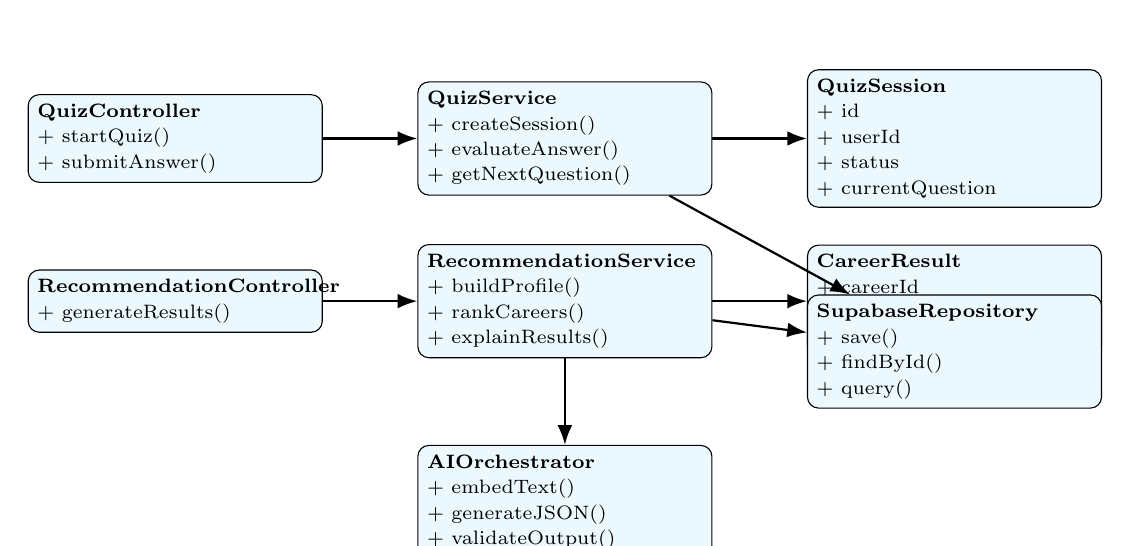
\begin{tikzpicture}[node distance=1.0cm and 1.0cm]
    \node[classbox] (qc)  {\textbf{QuizController}\\+ startQuiz()\\+ submitAnswer()};
    \node[classbox,right=1.2cm of qc]  (qs)  {\textbf{QuizService}\\+ createSession()\\+ evaluateAnswer()\\+ getNextQuestion()};
    \node[classbox,right=1.2cm of qs]  (qsm) {\textbf{QuizSession}\\+ id\\+ userId\\+ status\\+ currentQuestion};
    \node[classbox,below=1.1cm of qc]  (rc)  {\textbf{RecommendationController}\\+ generateResults()};
    \node[classbox,right=1.2cm of rc]  (rs)  {\textbf{RecommendationService}\\+ buildProfile()\\+ rankCareers()\\+ explainResults()};
    \node[classbox,right=1.2cm of rs]  (cr)  {\textbf{CareerResult}\\+ careerId\\+ matchScore\\+ explanation};
    \node[classbox,below=1.1cm of rs]  (ai)  {\textbf{AIOrchestrator}\\+ embedText()\\+ generateJSON()\\+ validateOutput()};
    \node[classbox,below=1.1cm of qsm] (repo){\textbf{SupabaseRepository}\\+ save()\\+ findById()\\+ query()};
    \draw[arrow] (qc) -- (qs);
    \draw[arrow] (qs) -- (qsm);
    \draw[arrow] (rc) -- (rs);
    \draw[arrow] (rs) -- (cr);
    \draw[arrow] (rs) -- (ai);
    \draw[arrow] (qs) -- (repo);
    \draw[arrow] (rs) -- (repo);
  \end{tikzpicture}}
  \caption{Simplified backend class diagram}
\end{figure}

\subsection{UI Design -- Wireframes}

This section presents the low-fidelity wireframes produced using Balsamiq during the design phase. These sketches were used to explore screen organization, navigation paths, and interaction flows before the implementation of the final mobile interface, and served as a shared visual reference for the development team.

\subsubsection{Authentication Screens}

\begin{figure}[H]
  \centering
  \IfFileExists{wireframes/wire_auth.png}{
    \includegraphics[width=0.92\linewidth]{wireframes/wire_auth.png}
  }{\figplaceholder[7cm]{%
    \textbf{Balsamiq Wireframes -- Login and Registration Screens}\\[6pt]
    Login: email field, password field, ``Login'' button, ``Forgot password?'' link\\
    Register: full name, email, password, confirm password, ``Create Account'' button}}
  \caption{Wireframes: authentication screens}
\end{figure}

\subsubsection{Home Dashboard}

\begin{figure}[H]
  \centering
  \IfFileExists{wireframes/wire_dashboard.png}{
    \includegraphics[width=0.55\linewidth]{wireframes/wire_dashboard.png}
  }{\figplaceholder[7cm]{%
    \textbf{Balsamiq Wireframe -- Home Dashboard}\\[6pt]
    User greeting banner, profile completion progress bar,\\
    quick-action cards: ``Take Quiz'', ``Upload CV'', ``My Recommendations''\\
    Recent activity section at the bottom}}
  \caption{Wireframe: home dashboard}
\end{figure}

\subsubsection{CV Upload Screen}

\begin{figure}[H]
  \centering
  \IfFileExists{wireframes/wire_cv.png}{
    \includegraphics[width=0.55\linewidth]{wireframes/wire_cv.png}
  }{\figplaceholder[7cm]{%
    \textbf{Balsamiq Wireframe -- CV Upload Screen}\\[6pt]
    File picker button (PDF only), drag-and-drop area,\\
    upload progress bar, extraction status indicator,\\
    summary of extracted skills after processing}}
  \caption{Wireframe: CV upload screen}
\end{figure}

\subsubsection{Adaptive Quiz Screen}

\begin{figure}[H]
  \centering
  \IfFileExists{wireframes/wire_quiz.png}{
    \includegraphics[width=0.55\linewidth]{wireframes/wire_quiz.png}
  }{\figplaceholder[7cm]{%
    \textbf{Balsamiq Wireframe -- Adaptive Quiz Screen}\\[6pt]
    Question text at top, multiple-choice option list,\\
    progress indicator ``Question N of 10'',\\
    ``Next'' button (disabled until an option is selected)}}
  \caption{Wireframe: adaptive quiz question screen}
\end{figure}

\subsubsection{Career Recommendations and Roadmap Screens}

\begin{figure}[H]
  \centering
  \IfFileExists{wireframes/wire_recommendations.png}{
    \includegraphics[width=0.92\linewidth]{wireframes/wire_recommendations.png}
  }{\figplaceholder[7cm]{%
    \textbf{Balsamiq Wireframes -- Recommendations and Roadmap}\\[6pt]
    Recommendations: ranked career cards (title, match \%, short explanation, chevron)\\
    Roadmap: phase list (Phase 1 / Phase 2 ...), skill gap tags, suggested resource links,\\
    estimated completion duration per phase}}
  \caption{Wireframes: career recommendations and learning roadmap}
\end{figure}

\subsubsection{Mentor Screen}

\begin{figure}[H]
  \centering
  \IfFileExists{wireframes/wire_mentor.png}{
    \includegraphics[width=0.92\linewidth]{wireframes/wire_mentor.png}
  }{\figplaceholder[7cm]{%
    \textbf{Balsamiq Wireframe -- Mentor Screen}\\[6pt]
    Mentor cards (photo, name, specialty, availability badge),\\
    ``Book Appointment'' button, appointment confirmation dialog,\\
    ``My Appointments'' list with status indicators}}
  \caption{Wireframes: mentor browsing and appointment booking}
\end{figure}

\subsection{Security and Risk Analysis}

Because MyPath processes personal, educational, and career-related data, security is an essential design concern. The main risks are: data privacy (CVs and profile data contain sensitive personal information), AI bias (recommendations may reflect imbalances in training data or prompt design), AI hallucination (LLM explanations may introduce unsupported claims), and unauthorized API access.

These risks are mitigated through authenticated access policies with encrypted data storage, AI output schema validation and constrained prompt templates, deterministic scoring for all critical recommendation logic, and token-based authentication with rate limiting on all API endpoints.

\subsection{Conclusion}

This chapter presented the full technical design of MyPath, covering its layered architecture, MVC backend organization, database schema, REST API contract, activity-based behavioral models, wireframe interface layout, and security considerations. The design combines deterministic processing with selective AI usage to achieve explainability, reliability, and maintainability, and serves as the direct foundation for the implementation described in the following chapter.

\clearpage

% ════════════════════════════════════════════════════════════════════════════
\section{Development and Prototype Solution}

This chapter presents the implementation of the proposed MyPath solution. It describes how the system design was translated into a functional prototype, covers the tools and technologies used, presents the implemented interfaces through final application screenshots, and documents the validation procedures applied to ensure system reliability.

\subsection{Introduction}

The development of MyPath focuses on building a functional prototype capable of delivering personalized career guidance through intelligent analysis and recommendation features. Based on the design presented in the previous chapter, the system is developed as a modular platform composed of frontend, backend, database, and AI-driven components. An incremental approach is followed: core functionalities are developed first and progressively extended with advanced features across six sprints.

\subsection{Development Details}

The development follows a modular and layered architecture implemented through successive sprints. The \textbf{frontend} is developed using React Native, providing a responsive mobile application covering all user-facing features. The \textbf{backend} is implemented in Python following MVC principles, handling API routing, request processing, and business coordination between the mobile frontend, Supabase services, and the AI orchestration module.

The \textbf{AI orchestration layer} supervises intelligent functionalities including prompt management, structured response control, and selective LLM interactions for explanation and personalization tasks, without replacing deterministic business logic. The \textbf{recommendation engine} combines CV and quiz data through deterministic scoring, with AI used only to generate explanatory text. The \textbf{roadmap generation module} implements a Hybrid Modular RAG pipeline, retrieving content from verified internal resources before AI-assisted personalization.

\subsection{Development Support}

\begin{table}[H]
\centering\small
\begin{tabular}{|p{3.5cm}|p{3.8cm}|p{6.2cm}|}
\hline
\textbf{Tool / Technology} & \textbf{Category} & \textbf{Usage} \\
\hline
React Native       & Frontend framework   & Mobile application development \\
Python / FastAPI   & Backend framework    & API development and service integration \\
Supabase           & BaaS                 & Authentication, PostgreSQL database, and file storage \\
Redis / BullMQ     & Cache and queue      & Asynchronous job processing and performance \\
External LLM APIs  & AI services          & Explanation generation and text personalization \\
Balsamiq           & UI prototyping       & Wireframe design \\
Jira               & Project management   & Sprint tracking and task organization \\
Git / GitHub       & Version control      & Code management and team collaboration \\
\hline
\end{tabular}
\caption{Development tools and technologies}
\end{table}

\subsection{Implementation}

\subsubsection{System Screens}

This section presents the final implemented screens of the MyPath mobile application. Each screen is accompanied by a description of its purpose and the functionality it provides.

\paragraph{Authentication Screens}

\begin{figure}[H]
  \centering
  \begin{subfigure}[b]{0.44\linewidth}
    \centering
    \IfFileExists{screens/login.png}{
      \includegraphics[width=\linewidth]{screens/login.png}
    }{\figplaceholder[9cm]{Login Screen\\(insert screenshot)}}
    \caption{Login screen}
  \end{subfigure}
  \hfill
  \begin{subfigure}[b]{0.44\linewidth}
    \centering
    \IfFileExists{screens/register.png}{
      \includegraphics[width=\linewidth]{screens/register.png}
    }{\figplaceholder[9cm]{Registration Screen\\(insert screenshot)}}
    \caption{Registration screen}
  \end{subfigure}
  \caption{Authentication screens: secure entry point with input validation and JWT-based authentication}
\end{figure}

\paragraph{Home Dashboard}

\begin{figure}[H]
  \centering
  \IfFileExists{screens/dashboard.png}{
    \includegraphics[width=0.48\linewidth]{screens/dashboard.png}
  }{\figplaceholder[9cm]{Home Dashboard Screen\\(insert screenshot)}}
  \caption{Home dashboard: displays user profile summary, recent results, and quick navigation to core features}
\end{figure}

\paragraph{CV Upload Screen}

\begin{figure}[H]
  \centering
  \IfFileExists{screens/cv_upload.png}{
    \includegraphics[width=0.48\linewidth]{screens/cv_upload.png}
  }{\figplaceholder[9cm]{CV Upload Screen\\(insert screenshot)}}
  \caption{CV upload screen: supports PDF submission with progress feedback and extraction status display}
\end{figure}

\paragraph{Adaptive Quiz Screens}

\begin{figure}[H]
  \centering
  \begin{subfigure}[b]{0.44\linewidth}
    \centering
    \IfFileExists{screens/quiz_question.png}{
      \includegraphics[width=\linewidth]{screens/quiz_question.png}
    }{\figplaceholder[9cm]{Quiz Question Screen\\(insert screenshot)}}
    \caption{Quiz question view}
  \end{subfigure}
  \hfill
  \begin{subfigure}[b]{0.44\linewidth}
    \centering
    \IfFileExists{screens/quiz_progress.png}{
      \includegraphics[width=\linewidth]{screens/quiz_progress.png}
    }{\figplaceholder[9cm]{Quiz Progress Screen\\(insert screenshot)}}
    \caption{Quiz progress indicator}
  \end{subfigure}
  \caption{Adaptive quiz screens: presents one question at a time with progress tracking across ten questions}
\end{figure}

\paragraph{Career Recommendations Screens}

\begin{figure}[H]
  \centering
  \begin{subfigure}[b]{0.44\linewidth}
    \centering
    \IfFileExists{screens/recommendations_list.png}{
      \includegraphics[width=\linewidth]{screens/recommendations_list.png}
    }{\figplaceholder[9cm]{Recommendations List\\(insert screenshot)}}
    \caption{Ranked career list}
  \end{subfigure}
  \hfill
  \begin{subfigure}[b]{0.44\linewidth}
    \centering
    \IfFileExists{screens/recommendation_detail.png}{
      \includegraphics[width=\linewidth]{screens/recommendation_detail.png}
    }{\figplaceholder[9cm]{Career Detail Screen\\(insert screenshot)}}
    \caption{Career detail with explanation}
  \end{subfigure}
  \caption{Recommendation screens: ranked careers with match percentages and AI-generated explanations}
\end{figure}

\paragraph{Roadmap Screen}

\begin{figure}[H]
  \centering
  \IfFileExists{screens/roadmap.png}{
    \includegraphics[width=0.48\linewidth]{screens/roadmap.png}
  }{\figplaceholder[9cm]{Roadmap Screen\\(insert screenshot)}}
  \caption{Roadmap screen: presents learning phases, identified skill gaps, and structured milestones toward the target career}
\end{figure}

\paragraph{Mentor Screens}

\begin{figure}[H]
  \centering
  \begin{subfigure}[b]{0.44\linewidth}
    \centering
    \IfFileExists{screens/mentor_list.png}{
      \includegraphics[width=\linewidth]{screens/mentor_list.png}
    }{\figplaceholder[9cm]{Mentor List Screen\\(insert screenshot)}}
    \caption{Mentor browsing}
  \end{subfigure}
  \hfill
  \begin{subfigure}[b]{0.44\linewidth}
    \centering
    \IfFileExists{screens/mentor_booking.png}{
      \includegraphics[width=\linewidth]{screens/mentor_booking.png}
    }{\figplaceholder[9cm]{Appointment Booking Screen\\(insert screenshot)}}
    \caption{Appointment booking}
  \end{subfigure}
  \caption{Mentor screens: browse mentors by specialty and schedule appointments}
\end{figure}

\subsubsection{Feature Implementation}

The main platform features were implemented and validated across multiple test scenarios.

The \textbf{CV analysis module} processes uploaded documents to extract skills, education, and experience into structured JSON records stored in the database. The \textbf{adaptive quiz module} maintains persistent sessions and progressively refines user profiling based on previous responses. The \textbf{recommendation engine} combines profile data with deterministic matching to produce ranked career suggestions, while the AI orchestration layer generates explanatory content. The \textbf{roadmap generation module} uses the Hybrid Modular RAG pipeline to produce structured, phase-based learning plans tailored to identified skill gaps. The \textbf{mentor module} supports appointment scheduling and integrates career opportunities from external sources into the mentor dashboard.

\subsection{Testing and Validation}

\subsubsection{Testing Strategy}

The testing strategy is multi-layered to address both deterministic modules and AI-assisted components:
\begin{itemize}
  \item \textbf{Unit testing:} verifies isolated backend services such as scoring functions and schema validators.
  \item \textbf{Integration testing:} evaluates communication between controllers, Supabase services, and the AI orchestration module.
  \item \textbf{API testing:} checks authentication behavior, input validation, and response conformity to JSON schemas.
  \item \textbf{Functional testing:} validates complete user journeys including registration, quiz completion, recommendation visualization, and roadmap consultation.
  \item \textbf{Qualitative AI review:} assesses whether generated explanations remain coherent, bounded, and aligned with deterministic recommendation evidence.
\end{itemize}

\subsubsection{Test Cases}

\begin{longtable}{|p{3cm}|p{3.8cm}|p{4.4cm}|p{2cm}|}
\hline
\textbf{Feature} & \textbf{Input} & \textbf{Expected Output} & \textbf{Result} \\
\hline
Authentication      & Valid credentials        & JWT token; redirect to dashboard         & Passed \\
Authentication      & Invalid password         & Access denied with error message         & Passed \\
Quiz session        & Start new quiz           & Session created; first question returned & Passed \\
Quiz progression    & Submit valid answer      & Answer stored; next question returned    & Passed \\
CV upload           & Valid PDF file           & Analysis job queued successfully         & Passed \\
CV parsing          & CV with skill keywords   & Structured skill list extracted          & Passed \\
Recommendation      & Completed quiz + CV data & Ranked career list with scores           & Passed \\
Roadmap generation  & Valid career result id   & Structured roadmap with phases           & Passed \\
Mentor booking      & Valid appointment data   & Appointment persisted as pending         & Passed \\
AI output control   & Recommendation evidence  & Explanation returned in valid JSON       & Passed \\
\hline
\caption{Test cases and results}
\end{longtable}

\subsection{Conclusion}

This chapter presented the development and validation of the MyPath prototype. The system was implemented incrementally following the Scrum methodology, and all major features were developed, integrated, and tested. The prototype demonstrates the feasibility of the proposed hybrid AI architecture and meets the main objectives defined in the specifications.

\clearpage

% ════════════════════════════════════════════════════════════════════════════
\section{General Conclusion \& Future Work}

\subsection{General Conclusion}

This project presented the design and development of MyPath, an AI-powered career recommendation platform aimed at assisting students and job seekers in making informed and personalized career decisions. The system integrates CV analysis, an adaptive quiz, a hybrid recommendation engine, a Hybrid Modular RAG-based roadmap generator, and a mentor interaction module into a unified, user-centered platform.

The proposed solution successfully addresses the limitations of traditional career guidance systems by delivering dynamic, data-driven, and personalized recommendations. The modular architecture ensures scalability and maintainability, while the hybrid design combining deterministic logic with controlled AI assistance improves both recommendation quality and system trustworthiness.

The development process, supported by Scrum methodology and modern tooling, produced a functional prototype that validates the feasibility of the proposed approach. Testing confirmed that all major features operate correctly and meet the defined requirements.

More broadly, this project demonstrates that academically rigorous AI-enabled software does not need to rely on unrestricted generative behavior. By combining structured engineering methods with selective AI assistance, MyPath illustrates a design pattern that is both technically credible and pedagogically valuable as a model for responsible AI integration in career guidance applications.

\subsection{Future Work}

Several enhancements can be considered to further extend the capabilities of MyPath. The mentor module can be enriched with performance tracking, reputation systems, and incentive-based features such as visibility ranking or certification badges to encourage greater professional engagement.

The platform can be extended to recommend certifications aligned with selected career paths and allow users to track their progress and achievements over time. Expanding the knowledge base with more detailed career pathways and industry-specific skill requirements would improve recommendation depth and accuracy.

From a technical perspective, further optimization of system performance and scalability would support a larger user base. Additional research-oriented extensions may include fairness audits of recommendation outputs, multilingual support, A/B testing of explanation styles, and longitudinal evaluation of whether roadmap adherence improves eventual employability outcomes.

\printbibliography

\end{document}
